
\chapter{Overzicht planning en fases}
\label{app:planning}

In de hierna volgende twee pagina's zijn de planning en fases in meer detail te omschreven\footnote{ Deze pagina's zijn in het engels geschreven, omdat dit de voertaal is binnen het bedrijf }. De onderzoekmethode, omschreven in de tabel \ref{tab:onderzoekmethode} op pagina \pageref{tab:onderzoekmethode}, dient als basis voor de planning.
\newline

In de "Breakdown structrure, estimates per activity"\ is de lijst met activiteiten omschreven zoals in \ref{sec:activiteiten} Activiteiten op pagina \pageref{sec:activiteiten}. De inschatting zijn te herleiden naar dagen. Dit is gedaan omdat dit beter aansluit bij de werkwijze van Shop2market. 
Verder wordt inzichtelijk gemaakt hoe de tijd is onderverdeeld per Proof of concept. Er wordt rekening gehouden met de mogelijke risico's en daarom kan in werkelijkheid de uitvoering sneller dan hier ingepland.
\newline

In "Visualisation in calendar days based on estimates per activity"\ is te zien de planning past binnen de iteraties van Shop2market, aansluitend bij de werkwijze in de organisatie.

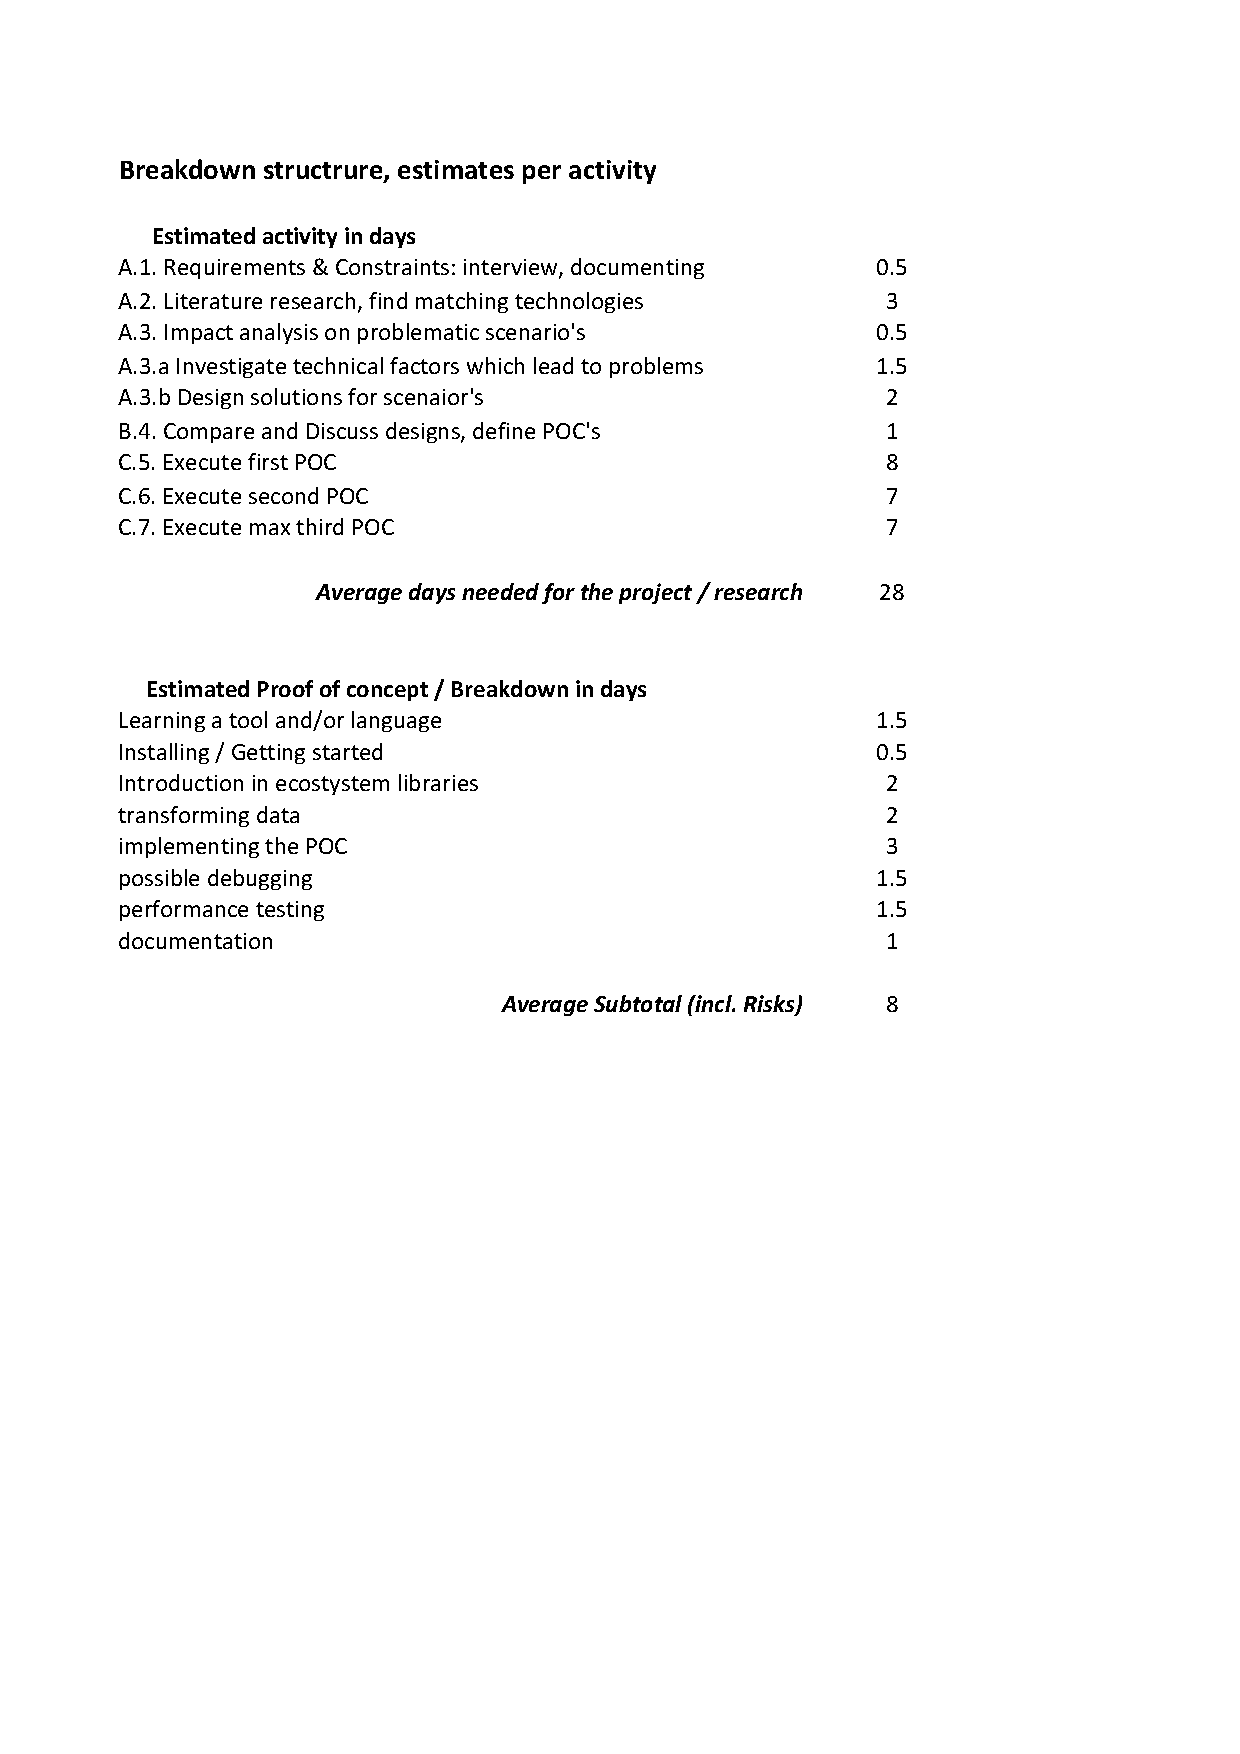
\includepdf[pages={1,2}]{appendix/planning-appendix-A.pdf}
